\documentclass[11pt,a4paper]{article}

% --- Essential Packages ---
\usepackage[utf8]{inputenc}
\usepackage[T1]{fontenc}
\usepackage{times}
\usepackage[margin=1in]{geometry}
\usepackage{amsmath,amssymb,amsfonts}
\usepackage{graphicx}
\usepackage{float}          % Enables strict [H] placement
\usepackage{booktabs}       % Professional table borders
\usepackage{tabularx}       % Auto-wrapping tables
\usepackage{multirow}       % Multirow cells
\usepackage{array}          % Enhanced column formatting
\usepackage{pifont}         % For clean checkmark (\ding{51}) and crossmark (\ding{55})
\usepackage{setspace}       % Line spacing
\usepackage[table,xcdraw]{xcolor}
\usepackage{titlesec}       % Custom section titles and spacing
\usepackage{caption}
\usepackage{subcaption}
\usepackage{enumitem}       % Tight itemize formatting
\usepackage{url}
\usepackage[hidelinks,colorlinks=true,linkcolor=blue,citecolor=blue,urlcolor=blue]{hyperref}

% --- Section Heading Formatting and Tight Spacing ---
\titleformat{\section}{\large\bfseries}{\thesection.}{0.5em}{}
\titleformat{\subsection}{\normalsize\bfseries}{\thesubsection.}{0.5em}{}
\titleformat{\subsubsection}{\normalsize\bfseries}{\thesubsubsection.}{0.5em}{}

\titlespacing*{\section}{0pt}{10pt plus 2pt minus 2pt}{2pt plus 1pt minus 1pt}
\titlespacing*{\subsection}{0pt}{8pt plus 2pt minus 2pt}{2pt plus 1pt minus 1pt}
\titlespacing*{\subsubsection}{0pt}{6pt plus 1pt minus 1pt}{1pt plus 1pt minus 1pt}

% --- Checkmarks and Crossmarks ---
\newcommand{\cmark}{\ding{51}}
\newcommand{\xmark}{\ding{55}}

% --- Figure path ---
\graphicspath{{figures/}{./}}

% --- Line Spacing & Paragraph Formatting ---
\setstretch{1.15}
\setlength{\parskip}{3pt plus 1pt minus 1pt}
\setlength{\parindent}{0pt}

% --- Custom column types for tabularx ---
\newcolumntype{L}{>{\raggedright\arraybackslash}X}
\newcolumntype{C}{>{\centering\arraybackslash}X}
\newcolumntype{R}{>{\raggedleft\arraybackslash}X}

\begin{document}

% --- Title Block (Anonymous: Authors Removed as Requested) ---
\begin{center}
    {\LARGE \textbf{GradeFormer: A Multi-Scale Slide-Graph Transformer with Low-Rank Attention Pooling for Cross-Institutional ISUP Grading of Prostate Biopsies} \par}
\end{center}

\vspace{1.5em}
\begin{abstract}
\noindent Prostate cancer management is strongly influenced by the International Society of Urological Pathology (ISUP) grade group, although histological grading remains subject to interobserver variation. Many weakly supervised whole-slide image (WSI) approaches represent a biopsy as an unordered collection of patches from a single scale and are evaluated within the cohort used for development.GradeFormer represents each tissue patch at two relative zoom levels: the complete patch (10$\times$) and a twice-zoomed central crop (20$\times$). Both views are encoded using a frozen UNI pathology foundation model and connected through intra-scale spatial k-nearest-neighbor and cross-scale correspondence edges. Three graph-transformer layers update the node features, after which 128 learnable latent queries perform low-rank attention (LRA) pooling to produce a continuous grade estimate. Development comprised 122 SICAPv2 biopsies from 76 patients and 244 Gleason2019 tissue-microarray cores assigned rule-derived pseudo-labels. A further 33 SICAPv2 biopsies from 19 patients were reserved for internal testing. External evaluation used 300 PANDA biopsies from two centers, without fine-tuning.Patient-grouped five-fold cross-validation produced a quadratic weighted kappa (QWK) of 0.860 (SD 0.039), while the held-out SICAPv2 set yielded a QWK of 0.946. On PANDA, QWK was 0.605 (95\% CI 0.531--0.673) with default rounding and 0.586 with out-of-fold (OOF)-derived cut-points; the corresponding patch-percentage baseline achieved 0.346 ($p < 0.001$). Exact or adjacent grades accounted for 78.3\% of external predictions, but errors were predominantly downward: 88 of 225 malignant biopsies were classified as benign, and none of the 33 ISUP 5 biopsies was correctly graded. Graph layers followed by mean pooling achieved an external QWK of 0.317, whereas LRA pooling without graph message passing reached 0.681. Additional LRA ensembles achieved QWK values of 0.623 and 0.690. Fold-model disagreement was only weakly associated with error ($r = 0.283$).LRA pooling was associated with substantially better cross-cohort stability than mean pooling. The graph message-passing layers did not improve external generalization over LRA pooling alone. Persistent under-grading in the external cohort, including the failure to identify any ISUP 5 biopsy, precludes clinical use and indicates the need for target-site calibration and larger, prospectively assembled external cohorts.
\end{abstract}

\vspace{0.5em}
\noindent \textbf{Keywords:} Computational pathology; Prostate cancer; Graph transformer; Multi-scale learning; Pathology foundation model; Ordinal regression; Cross-institutional generalization; Uncertainty triage

\vspace{1em}

\section{Introduction}
Prostate cancer is the second most frequently diagnosed cancer in men worldwide, after lung cancer \cite{ref1}. Decisions about active surveillance, surgery, radiotherapy, and androgen-deprivation therapy are informed in large part by the ISUP grade group \cite{ref2, ref3}. This grading system translates the primary and secondary Gleason growth patterns, which range from well-formed glands to fused, cribriform, and solid tumor structures, into five prognostic groups. Benign tissue is represented as grade 0 in the present study. Despite its clinical importance, grading remains a visual assessment of gigapixel hematoxylin-and-eosin (H\&E)-stained sections, and agreement between observers is imperfect, including among specialist uropathologists \cite{ref4}. In the multi-reader cohort underlying Gleason2019, pairwise agreement among six pathologists ranged from 0.45 to 0.62 in unweighted $\kappa$ \cite{ref5}. Disagreement reflects, among other factors, the gradual transition between adjacent growth patterns, intrabiopsy tumor heterogeneity, and the subjective estimation of pattern proportions.

Whole-slide imaging has created opportunities to support histological assessment with computational methods. In the PANDA challenge, several algorithms achieved agreement with expert reference standards comparable to that of pathologists on independent validation cohorts \cite{ref6}. The scale of a WSI, however, makes direct processing of every pixel impractical. Most systems therefore use multiple instance learning (MIL) \cite{ref7, ref8}, encoding tissue patches and combining their representations into a slide-level prediction through a permutation-invariant aggregation function. Attention-based pooling \cite{ref7} and clustering-constrained attention \cite{ref8} are established examples. Although effective across many pathology tasks, conventional MIL pipelines leave several issues relevant to ordinal prostate grading unresolved:

\begin{itemize}[leftmargin=1.8em, itemsep=3pt, parsep=0pt]
  \item \textbf{Spatial relationships are often omitted.} Set-based aggregation treats patch embeddings as independent instances, whereas pathologists interpret glands and tumor architecture across neighboring fields. This continuity can help distinguish discrete Gleason pattern 3 (GP3) glands from poorly formed or cribriform pattern 4 (GP4) structures. Graph-based and correlation-aware approaches, including Patch-GCN \cite{ref9} and TransMIL \cite{ref10}, incorporate contextual information, but their use for ordinal prostate grading remains limited.
  \item \textbf{A single image scale may not capture all diagnostic cues.} Low-power review (approximately 5$\times$ or 10$\times$) supports assessment of glandular architecture, stromal--epithelial relationships, and tumor extent. Higher-power inspection (20$\times$ or 40$\times$) provides finer detail about nuclei and luminal boundaries. A single-scale representation must compress these complementary observations into one feature vector.
  \item \textbf{Nominal classification losses do not encode grade distance.} ISUP groups represent an ordered scale of disease aggressiveness, yet conventional softmax cross-entropy penalizes an ISUP 1-to-2 error in the same way as an ISUP 1-to-5 error. This does not reflect the squared distance weighting used by quadratic weighted kappa (QWK) \cite{ref11}.
  \item \textbf{Internal validation alone provides limited evidence of transportability.} Many systems are evaluated using random partitions of one cohort, such as the 155 biopsies in SICAPv2 \cite{ref12}. Such experiments cannot establish how performance changes with differences in tissue processing, section preparation, staining, or scanner characteristics across institutions.
\end{itemize}

We developed GradeFormer to investigate multi-scale and spatial representations for ordinal ISUP grading under cross-institutional domain shift. Each tissue location is represented by a full-patch view and a central crop at twice the relative zoom; both are encoded by the frozen UNI vision transformer (ViT-L/16) \cite{ref13}. The resulting features are arranged in a graph containing spatial k-nearest-neighbor connections within each scale and correspondence edges between scales. Three graph-transformer layers update the node representations, and 128 learnable latent queries aggregate the nodes through LRA pooling. A regression head predicts a continuous grade score. Discrete grades are obtained using either default rounding or cut-points estimated from pooled out-of-fold (OOF) predictions, without using the held-out SICAPv2 or PANDA labels for cut-point fitting.

The contributions of this work are fourfold:

\begin{itemize}[leftmargin=1.8em, itemsep=3pt, parsep=0pt]
  \item \textbf{Multi-scale slide graph.} A two-scale slide graph is constructed by connecting spatial neighbors ($k = 8$) within each view and linking the two representations of each patch location. This design allows the model to combine architectural and cytological information. Graph-based and hierarchical WSI methods have been reported previously \cite{ref9, ref14}; the present study applies a multi-scale graph design to ordinal prostate grading and examines its behavior under domain shift.
  \item \textbf{Ordinal regression with out-of-fold calibration.} The grading task is formulated as continuous regression with a mean-squared-error objective. Grade thresholds are estimated using only the pooled OOF predictions from the development cross-validation, and performance is reported with both these thresholds and conventional rounding.
  \item \textbf{Pooling under domain shift.} The ablation experiments reveal a marked difference between pooling strategies under external evaluation. Graph-transformer layers followed by mean pooling achieved a PANDA QWK of 0.317, whereas LRA pooling without graph layers achieved 0.681. We refer to this empirical pattern as the ``Pooling Paradox''. Because the comparisons are not fully factorial, it is treated as an observation rather than evidence for a specific mechanism.
  \item \textbf{External evaluation and error analysis.} The external analysis covers 300 PANDA biopsies evaluated without fine-tuning and includes error direction, error severity, and fold-ensemble disagreement. Although 78.3\% of predictions were exact or adjacent to the reference grade, downward errors were common. The association between ensemble disagreement and absolute error was weak ($r = 0.283$), limiting its value as a stand-alone referral signal.
\end{itemize}

Section 2 summarizes related work. Section 3 describes the datasets, preprocessing pipeline, architecture, and training protocol. Section 4 presents internal and external performance, ablation and encoder comparisons, multi-seed analyses, error-severity results, and exploratory interpretability findings. Section 5 discusses the implications and limitations, followed by the conclusion in Section 6.


\section{Related Work}

\subsection{Structure-Aware Multiple Instance Learning}
MIL is widely used to learn slide-level predictions from weakly labeled histopathology images. Attention-based MIL (ABMIL) assigns gated attention weights to patch embeddings, providing an efficient aggregation mechanism and a way to inspect instance contributions \cite{ref7}. CLAM extends this framework with instance-level clustering constraints that encourage separation of class-related evidence \cite{ref8}. Neither approach explicitly represents the spatial position of each patch. Graph neural networks offer a means of incorporating such relationships: graph convolutional networks \cite{ref15} and graph attention networks \cite{ref16} provide the underlying message-passing operations, while Patch-GCN constructs a graph over WSI patches and propagates information between spatial neighbors \cite{ref9}. TransMIL models correlations among instances using self-attention over a structured token sequence, without relying on explicit spatial coordinates \cite{ref10}. HIPT aggregates representations hierarchically across image resolutions \cite{ref14}. These methods establish several ways to capture context, but their performance under cross-institutional distribution shifts remains less extensively characterized than their within-cohort performance.


\subsection{Pathology Foundation Models and Vision Transformers}
Histopathology encoders have increasingly moved beyond ImageNet-supervised convolutional networks toward self-supervised models trained on large collections of tissue images. Phikon, introduced by Filiot et al. \cite{ref17}, uses a ViT-Base architecture pretrained with iBOT, a masked-image-modeling approach, on more than 40 million histology images spanning 16 cancer types. UNI, reported by Chen et al. \cite{ref13}, is a ViT-L/16 model pretrained on more than 100 million tissue patches from over 100,000 diagnostic WSIs. These models provide transferable patch-level representations, but slide-level inference still depends on how patch features are aggregated. The aggregation strategy may therefore influence robustness when the target institution differs from the development cohort.


\subsection{Computational Prostate Grading Pipelines}
Automated prostate biopsy grading has been examined using datasets that include SICAPv2 and PANDA. Silva-Rodríguez et al. \cite{ref12} introduced SICAPv2 alongside a patch-level convolutional model trained from scratch. Its three convolutional blocks used global max pooling, and patch-level grade proportions were passed to a multilayer perceptron for biopsy-level scoring; the reported test-subset quadratic $\kappa$ was 0.81. Marini et al. \cite{ref18} addressed between-center color variation with data-driven color augmentation (DDCA), which filters augmented images against a reference collection containing more than two million H\&E color variations. For hue--saturation--contrast (HSC) augmentation applied to 750$\times$750 prostate patches extracted at 40$\times$ and resized to 224$\times$224, the reported patch-level $\kappa$ was 0.717 $\pm$ 0.048 on the internal SICAPv2 test partition and 0.492 $\pm$ 0.061 on the external PANDA partition. These values indicate that color augmentation alone did not eliminate the observed domain gap. Schmidt et al. \cite{ref19} proposed attention Gaussian processes (AGP) for probabilistic MIL attention, using 512$\times$512 patches at 10$\times$ with 50\% overlap. AGP achieved a quadratic $\kappa$ of 0.847 $\pm$ 0.001 on SICAPv2 (mean $\pm$ standard error across four runs of four-fold cross-validation). In the reverse transfer direction, models trained on PANDA and evaluated on all SICAPv2 images under ISUP grading reached 0.920 $\pm$ 0.001. Dominguez-Morales et al. \cite{ref1} compared fully supervised, semi-supervised, and weakly supervised methods, including ABMIL, TransMIL, and CLAM, across nine Gleason datasets. Fully supervised approaches performed best for Gleason grading, whereas CLAM performed best for Gleason scoring.

Table 1 places these studies alongside GradeFormer. The earlier pipelines summarized here use a single magnification and do not explicitly combine multi-scale features with spatial graph modeling. GradeFormer brings together two relative scales, graph-based context, latent-query pooling, and an ordinal regression objective. The studies differ in cohort composition, train--test partitioning, label definition, evaluation unit, and reported metric; the GradeFormer development folds also include Gleason2019 cores with pseudo-labels. Table 1 should therefore be read as a descriptive overview, not as a direct comparison of methods.


\begin{table}[H]
\centering
\small
\setlength{\tabcolsep}{3.5pt}
\renewcommand{\arraystretch}{1.25}
\caption{Overview of prostate histopathology grading methods, datasets, preprocessing, and evaluation settings. ``Ext. Val.'' indicates evaluation on a cohort not used for training; ``MS / Graph'' indicates multi-scale representation and spatial graph modeling.}
\label{tab:related_methods}
\begin{tabularx}{\textwidth}{p{2.2cm} p{1.6cm} p{2.3cm} X c c p{2.3cm}}
\toprule
\textbf{Reference} & \textbf{Dataset} & \textbf{Preprocessing} & \textbf{Method} & \textbf{\shortstack{Ext.\\Val.}} & \textbf{\shortstack{MS /\\Graph}} & \textbf{\shortstack{QWK / $\kappa$\\(int. / ext.)}} \\
\midrule
Silva-Rodr\'iguez et al. (2020)~\cite{ref12} & SICAPv2 & Patch-based WSI processing & Shallow CNN trained from scratch + global max pooling; MLP on grade percentages & \xmark & \xmark~/\ \xmark & 0.81 / --- \\
\addlinespace
Marini et al. (2023)~\cite{ref18} & SICAPv2, PANDA & $750\times 750$ patches at 40$\times$, resized to $224\times 224$ & Data-driven HSC colour augmentation & \cmark & \xmark~/\ \xmark & 0.717 $\pm$ 0.048 / \newline 0.492 $\pm$ 0.061 \\
\addlinespace
Schmidt et al. (2024)~\cite{ref19} & SICAPv2, PANDA & 10$\times$ mag.; $512\times 512$ patches; 50\% overlap & Attention Gaussian process (AGP) MIL & \cmark & \xmark~/\ \xmark & 0.847 $\pm$ 0.001$^\dagger$ / \newline 0.920 $\pm$ 0.001 \\
\addlinespace
\textbf{GradeFormer (this work)} & SICAPv2 + Gleason2019 (dev); PANDA (test) & Otsu filtering, Macenko norm., two-view tiling & Multi-scale graph transformer + LRA pooling & \cmark & \cmark~/\ \cmark & \textbf{0.860 / 0.605} \\
\bottomrule
\end{tabularx}
\end{table}


\subsection{Ordinal Regression Formulations}
Standard multi-class cross-entropy treats grades as unrelated categories and does not distinguish near misses from errors spanning several grade levels. Ordinal approaches instead represent the ordering of the target classes. Examples include cumulative-link models, rank-consistent binary decompositions such as CORAL \cite{ref20}, and regression to a continuous score. We use continuous-score regression with mean-squared error (MSE), then map the output to an integer grade using decision thresholds. Although MSE is not identical to the QWK objective, it penalizes larger numerical deviations more strongly than smaller ones and is therefore compatible with the ordered structure of the target.


\section{Materials and Methods}
The workflow is summarized in Figure 1. Candidate tissue regions are separated from background and stain variation is reduced through color normalization. Each retained patch is represented at two relative zoom levels and encoded with a frozen pathology foundation model. The resulting features are assembled into a slide graph, updated by graph-transformer layers, and summarized by LRA pooling. A regression head predicts a continuous ISUP score, which is converted to a discrete grade using the selected thresholding rule.


\begin{figure}[H]
\centering
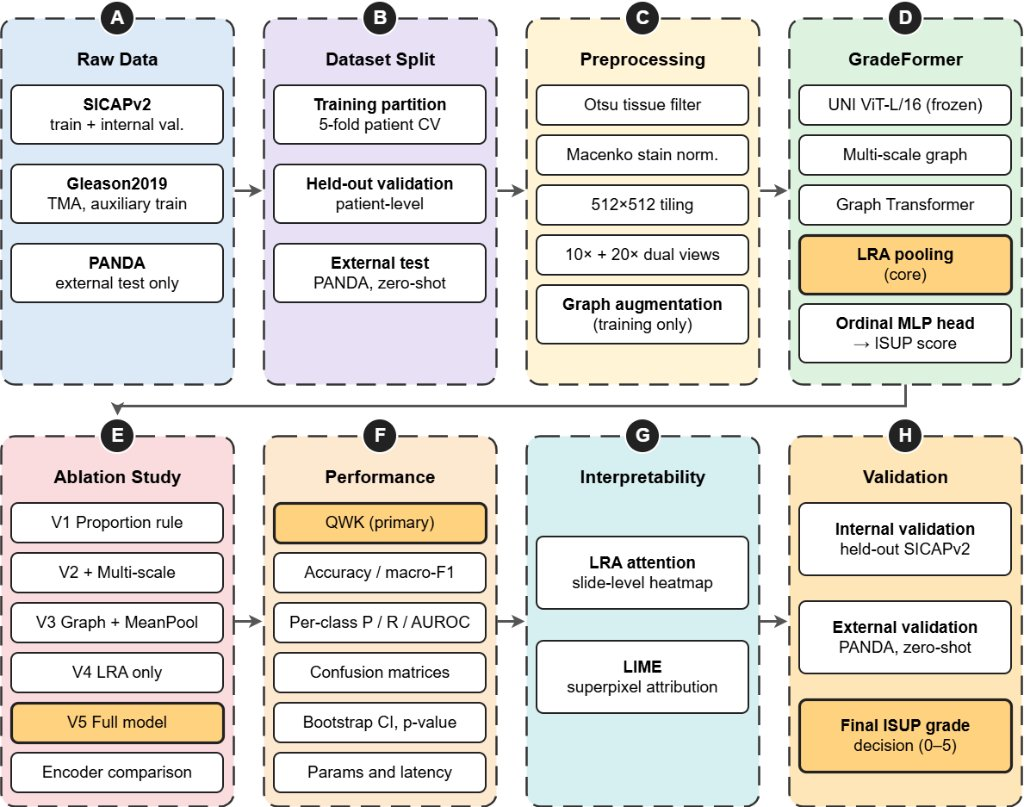
\includegraphics[width=\textwidth]{figure1.png}
\caption{GradeFormer workflow. (A) Data: SICAPv2 (training and internal validation), Gleason2019 (auxiliary training) and PANDA (external test only). (B) Split: patient-level five-fold cross-validation, a held-out SICAPv2 set and an external PANDA test set. (C) Preprocessing: Otsu tissue filtering, Macenko normalization, 512$\times$512 tiling, two views per patch (10$\times$ and 20$\times$, relative zoom levels) and graph augmentation during training only. (D) Model: frozen UNI ViT-L/16 encoder, multi-scale graph, graph transformer, LRA pooling and an ordinal MLP head. (E) Ablation variants V1--V5 and an encoder comparison. (F) Metrics: QWK (primary), accuracy, macro-F1, per-class metrics, bootstrap CIs, and parameter count and latency. (G) Interpretability: slide-level LRA attention heatmaps and patch-level LIME attributions. (H) Internal and external validation and the final ISUP grade (0--5).}
\label{fig:workflow}
\end{figure}


\subsection{Datasets}
Three publicly available prostate histopathology datasets were used: SICAPv2 \cite{ref12}, Gleason2019 \cite{ref5}, and PANDA \cite{ref6}. Their roles, analysis units, label sources, and patch sources are summarized in Table 2.


\begin{table}[H]
\centering
\small
\setlength{\tabcolsep}{3pt}
\renewcommand{\arraystretch}{1.25}
\caption{Datasets used for model development, auxiliary supervision, internal testing, and external evaluation.}
\label{tab:datasets}
\begin{tabularx}{\textwidth}{p{1.6cm} p{2.2cm} p{2.0cm} p{1.7cm} p{1.8cm} X p{2.1cm}}
\toprule
\textbf{Dataset} & \textbf{Role} & \textbf{\shortstack{Unit of\\analysis}} & \textbf{\shortstack{Slides /\\cores}} & \textbf{Patients} & \textbf{\shortstack{Ground-truth\\source}} & \textbf{\shortstack{Patch\\source}} \\
\midrule
SICAPv2~\cite{ref12} & Development (122) and held-out internal test (33) & Whole-slide biopsy & 155 & 95 & Primary and secondary Gleason pattern per slide (\texttt{wsi\_labels} file) & $512\times 512$ patches from official partition files \\
\addlinespace
Gleason2019~\cite{ref5} & Auxiliary development data only & Tissue microarray (TMA) core & 244 & Not given per core (full cohort: 333 cores, 231 patients) & STAPLE consensus of pathologist annotations; core grade from percentage rule (Section 3.3) & $512\times 512$ tiles cut from released core images \\
\addlinespace
PANDA~\cite{ref6} & External test only & Whole-slide biopsy & 300 (149 Karolinska, 151 Radboud) & Not reported & ISUP grade provided with PANDA training metadata & $512\times 512$ tiles at pyramid level 0 \\
\bottomrule
\end{tabularx}
\end{table}


\subsection{Primary Development and Internal Validation: SICAPv2}
SICAPv2 \cite{ref12} contains 155 prostate biopsy WSIs from 95 patients treated at Hospital Clínico Universitario de Valencia, Spain. The release includes patch-level Gleason pattern labels (non-cancerous, GP3, GP4, and GP5) and slide-level primary and secondary Gleason patterns. We used the 12,081 patches of 512$\times$512 pixels supplied in the official partition files and obtained slide-level pattern information from the accompanying \texttt{wsi\_labels} file. For each biopsy, the ISUP grade group g $\in$ {0, 1, 2, 3, 4, 5} was derived from its reported primary (p) and secondary (s) Gleason patterns according to Equation (1):


\begin{equation}
g(p, s) = 
\begin{cases} 
0 & \text{if } p < 3 \text{ or } s < 3 \\
1 & \text{if } p + s \le 6 \\
2 & \text{if } p = 3, s = 4 \\
3 & \text{if } p = 4, s = 3 \\
4 & \text{if } p + s = 8 \\
5 & \text{if } p + s \ge 9 
\end{cases}
\label{eq:isup_mapping}
\end{equation}

In this expression, p and s $\in$ {0, 3, 4, 5} denote the primary and secondary patterns, with 0 indicating benign tissue; g is the resulting grade group used as the SICAPv2 supervision target \cite{ref2, ref3}.


\subsection{Auxiliary Development Data: Gleason2019}
The Gleason2019 release for the MICCAI 2019 Grand Challenge contains 244 training tissue-microarray (TMA) cores with pixel-level Gleason annotations and STAPLE consensus maps \cite{ref5}. The broader multi-reader cohort comprised 333 TMA cores from 231 radical-prostatectomy patients, annotated by six pathologists. We divided each of the 244 available cores into non-overlapping 512$\times$512 tiles and retained up to 60 tissue-containing tiles per core, yielding 14,526 tiles. Each tile was assigned the majority STAPLE class within its area. Core-level pseudo-grades were then derived from the relative frequencies of GP3, GP4, and GP5 among malignant tiles. Cores without malignant tiles were assigned grade 0. For the remaining cores, patterns represented in more than 5\% of malignant tiles were ranked by frequency; the most frequent pattern was designated primary, and the second most frequent (or the primary pattern again when no second pattern met the threshold) was designated secondary. If no pattern exceeded 5\%, the most frequent pattern was used. The resulting pair was mapped using the fixed lookup implemented in the analysis pipeline: 3+3→1, 3+4→2, 4+3→2, 4+4→3, 3+5→3, 5+3→3, 4+5→4, 5+4→4, and 5+5→5. This mapping differs from the ISUP definitions in Equation (1): under the ISUP scheme, 4+3 corresponds to grade 3; 4+4, 3+5, and 5+3 correspond to grade 4; and 4+5 and 5+4 correspond to grade 5. The implemented lookup therefore assigns pseudo-grades one level below the ISUP grade for these pattern combinations, introducing a systematic downward bias into part of the auxiliary supervision. The same lookup was used for the patch-percentage baseline in Section 4.4. Gleason2019 cores were included only in the development pool to broaden the range of tissue appearance; they were not used in the held-out SICAPv2 or PANDA evaluations, although they were represented in the development cross-validation folds.


\subsection{Patient-Stratified Data Partitioning}
Because SICAPv2 includes multiple biopsies from some patients, partitioning at the slide level could place samples from the same patient in both training and validation sets. We therefore divided the 95 patients into development and held-out groups using an 80:20 split. The development partition contained 76 patients and 122 biopsies; the held-out partition contained 19 patients and 33 biopsies. Stratification was based on each patient's most frequent patch-level class. The 244 Gleason2019 cores were then added to the 122 development biopsies, creating a 366-slide pool. Five-fold cross-validation within this pool was grouped by patient: each Gleason2019 core was treated as an independent group, resulting in 320 groups, and stratification used each group's majority grade. Cross-validation informed early stopping, model selection, and OOF cut-point estimation. The 33 held-out SICAPv2 biopsies were excluded from all of these steps.


\subsection{Tissue Foreground Segmentation and Filtering}
To exclude blank glass and background regions, we applied Otsu thresholding \cite{ref21} to the grayscale image of each candidate tile. The selected threshold, $\tau$*, minimizes within-class intensity variance, as expressed in Equation (2):


\begin{equation}
\tau^* = \arg\min_\tau \left[ \omega_0(\tau) \cdot \sigma_0^2(\tau) + \omega_1(\tau) \cdot \sigma_1^2(\tau) \right]
\label{eq:otsu}
\end{equation}

Here, $\tau$ $\in$ [0, 255] is the grayscale threshold; ω₀($\tau$) and ω₁($\tau$) are the proportions of pixels assigned to background and tissue; and $\sigma$₀²($\tau$) and $\sigma$₁²($\tau$) are their respective variances. Gleason2019 and PANDA tiles containing less than 5\% tissue were discarded. SICAPv2 patches were used as supplied in the official partition files and were not subjected to additional filtering.


\subsection{Macenko Stain Normalization}
Differences in slide preparation, staining batches, and scanner response can alter H\&E appearance across institutions. We therefore normalized all patches and tiles using the optical-density procedure described by Macenko et al. \cite{ref22}, implemented through the staintools package with luminosity standardization. RGB values were converted to optical density; the hematoxylin and eosin stain vectors were estimated from the 1st and 99th percentiles of the angular distribution in the subspace spanned by the two leading singular vectors; and stain concentrations were then expressed in a reference stain basis. The reference was a single patch from the SICAPv2 development set. This procedure targets color variation while retaining the underlying tissue structure.


\subsection{Multi-Scale Patch Representation}
Each normalized 512$\times$512 patch was converted into two co-registered views to represent tissue architecture and finer cellular detail (Equation 3):


\begin{equation}
X(10\times) = \text{Resize}(X, d), \quad X(20\times) = \text{Resize}(\text{Crop}_{256}(X), d)
\label{eq:multiscale}
\end{equation}

The coarse view, X⁽¹⁰ˣ⁾, comprises the complete patch resized to the encoder input of 224$\times$224 pixels. It preserves the broader glandular arrangement. The fine view, X⁽²⁰ˣ⁾, is obtained by cropping the central 256$\times$256 region and resizing it to the same input dimensions; this view covers one-quarter of the original area and provides twice the relative zoom. The labels 10$\times$ and 20$\times$ therefore denote the zoom relationship between the two views rather than calibrated optical magnifications. The physical field of view represented by a 512$\times$512 patch varies with the source resolution, which differs among SICAPv2 patches, Gleason2019 tiles, and PANDA level-0 tiles.


\subsection{External Evaluation: PANDA}
Cross-institutional performance was assessed on 300 biopsies from the PANDA challenge \cite{ref6}. These were the first 300 entries in the public PANDA training metadata file, ordered by anonymized hexadecimal image identifier; selection was neither randomized nor class-balanced. The subset comprised 149 slides from Karolinska Institutet (Stockholm, Sweden) and 151 from Radboud University Medical Center (Nijmegen, the Netherlands). Reference grades were taken from the \texttt{isup\_grade} field in the PANDA training metadata. These are the public training labels and should not be conflated with the expert-panel reference standards used for the challenge's blinded validation cohorts \cite{ref6}. Each WSI was tiled at pyramid level 0 into non-overlapping 512$\times$512 regions. Tiles were filtered and normalized as described above, and up to 384 tissue-containing tiles per slide were retained in raster order. No PANDA images, tiles, or features were used for model training, model selection, hyperparameter search, or OOF cut-point fitting. The grade distributions of the development, held-out, and external cohorts are reported in Table 3.


\begin{table}[H]
\centering
\small
\renewcommand{\arraystretch}{1.15}
\caption{Biopsy-level ISUP grade distribution in the 366-slide development pool (122 SICAPv2 biopsies with reference grades and 244 Gleason2019 cores with pseudo-grades), the 33-biopsy held-out SICAPv2 cohort, and the 300-biopsy PANDA external cohort.}
\label{tab:cohort_distribution}
\begin{tabularx}{\textwidth}{lCCC}
\toprule
\textbf{ISUP grade} & \textbf{Development pool ($n = 366$)} & \textbf{Held-out SICAPv2 ($n = 33$)} & \textbf{PANDA external ($n = 300$)} \\
\midrule
0 (benign) & 51 & 9 & 75 \\
1 & 68 & 5 & 80 \\
2 & 79 & 3 & 38 \\
3 & 115 & 3 & 39 \\
4 & 21 & 1 & 35 \\
5 & 32 & 12 & 33 \\
\midrule
\textbf{Total} & \textbf{366} & \textbf{33} & \textbf{300} \\
\bottomrule
\end{tabularx}
\end{table}


\subsection{GradeFormer Architecture}
As illustrated in Figure 2, GradeFormer comprises six processing stages: (i) dual-scale concentric patch extraction; (ii) frozen foundation-model encoding of the two patch views; (iii) construction of a multi-scale spatial graph containing within-scale spatial links and cross-scale correspondences; (iv) contextual feature updates through graph-transformer layers; (v) Low-Rank Attention (LRA) pooling to obtain a fixed-length slide representation; and (vi) continuous ordinal regression, followed by conversion to discrete ISUP grades.


\begin{figure}[H]
\centering
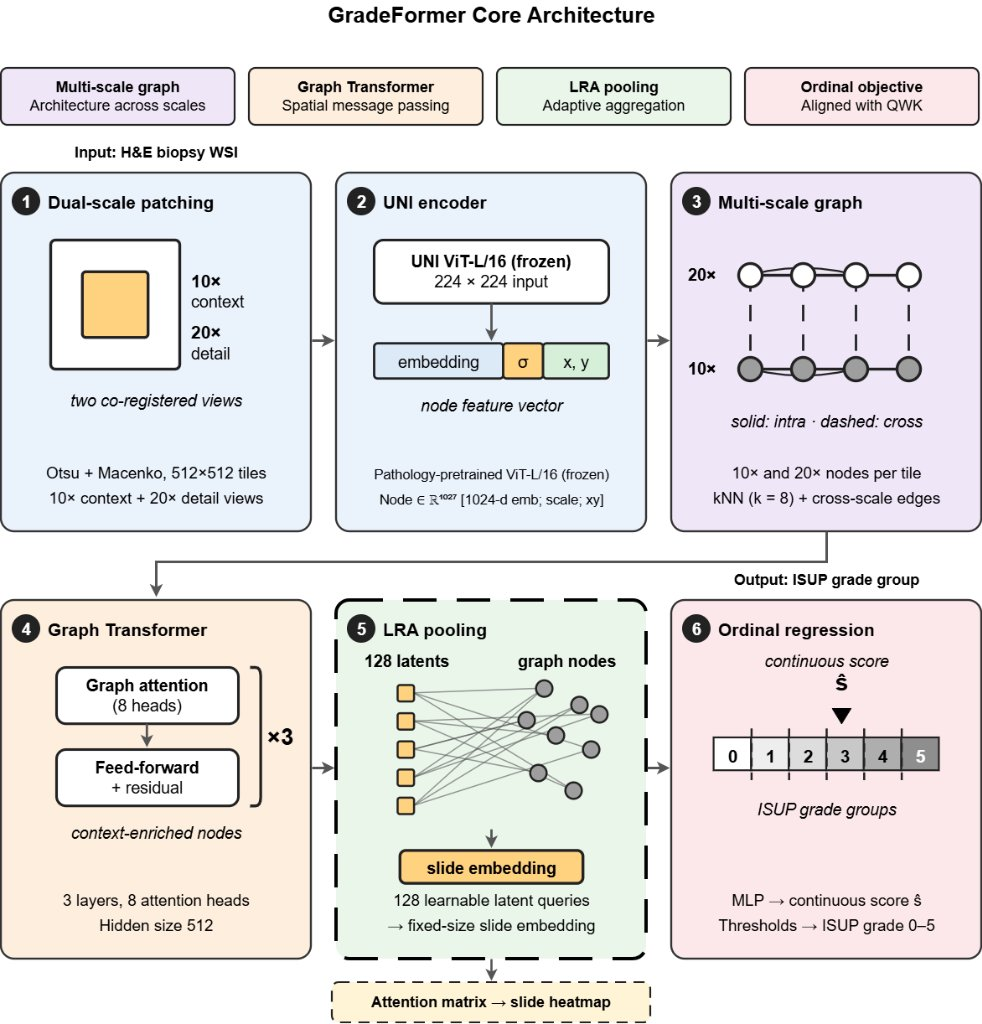
\includegraphics[width=\textwidth]{figure2.png}
\caption{GradeFormer architecture. Stage 1 extracts concentric and patch views. Stage 2 embeds each view using the frozen UNI ViT-L/16 backbone, appends normalized spatial coordinates and scale flags, and applies an input projection. Stage 3 constructs a slide graph with intra-scale $k$-nearest-neighbor and cross-scale correspondence edges. Stage 4 applies three graph-transformer layers with residual connections, layer normalization, and dropout. Stage 5 aggregates node features through low-rank attention (LRA) pooling with 128 learnable latent queries. Stage 6 predicts a continuous grade through a two-layer ordinal MLP head, mapped to discrete ISUP grades by thresholding.}
\label{fig:architecture}
\end{figure}


\subsubsection{Feature Extraction with the Frozen UNI Foundation Model}
For each patch location i $\in$ {1, …, N}, the coarse view X⁽¹⁰ˣ⁾ᵢ and fine view X⁽²⁰ˣ⁾ᵢ are independently passed through UNI (ViT-L/16, 303.4 M parameters) \cite{ref13, ref23}, as specified in Equation (4). The 24 transformer blocks remain frozen. This avoids adapting a high-capacity encoder to a relatively small cohort and makes feature extraction feasible with the available NVIDIA T4 GPU. The 1024-dimensional class-token representation is retained as the embedding for each view.


\begin{equation}
e_i^{(10\times)} = f_\theta(X_i^{(10\times)}), \quad e_i^{(20\times)} = f_\theta(X_i^{(20\times)})
\label{eq:embedding}
\end{equation}

Two linear probes were additionally fitted to the frozen features using patch-level labels. The benign-versus-malignant probe achieved a best held-out AUROC of 0.968 and accuracy of 0.879; the three-class GP3/GP4/GP5 probe achieved QWK 0.654 and macro AUROC 0.880. These probes do not modify the features supplied to the graph model. They are used only for the patch-percentage baseline (Section 4.4) and the LIME analysis (Section 4.9). Before graph construction, each embedding is augmented with a scale indicator $\sigma$ $\in$ {0, 1} (0 for the coarse view and 1 for the fine view) and two normalized patch coordinates. Coordinates are centered on the slide centroid and scaled by the largest Chebyshev distance, as shown in Equation (5):


\begin{equation}
\tilde{\mathbf{c}}_i = \frac{(r_i, c_i) - (\bar{r}, \bar{c})}{\max_j \|(r_j, c_j) - (\bar{r}, \bar{c})\|_\infty}, \quad \mathbf{x}_i = \left[ e_i^{(10\times)}; e_i^{(20\times)}; \tilde{\mathbf{c}}_i; \sigma \right] \in \mathbb{R}^{1027}
\label{eq:norm_coords}
\end{equation}

Here, (rᵢ, cᵢ) are the patch-grid coordinates, (r̄, c̄) is their mean, c̃ᵢ $\in$ [−1, 1]² denotes the normalized position, and xᵢ is the resulting 1027-dimensional input vector: 1024 embedding components, one scale indicator, and two coordinate values.


\subsubsection{Multi-Scale Slide-Graph Construction}
For a slide containing N patch locations, we define a graph $\mathcal{G}$ = ($\mathcal{V}$, $\mathcal{E}$) with |$\mathcal{V}$| = 2N nodes. The first N nodes, u₁, …, uN, represent the coarse views; the remaining N nodes, uN+1, …, u2N, represent the corresponding fine views. The edge set contains two connection types:

\noindent \textbf{Intra-scale spatial edges ($\mathcal{E}$intra).} At each scale $\sigma$ $\in$ {0, 1}, every node is connected to its k nearest neighbors according to Euclidean distance between patch locations (Equation 6), with $k = 8$ and no self-loops. These edges provide a route for contextual information to pass between nearby tissue regions.


\begin{equation}
\mathcal{E}_{\text{intra},\sigma} = \left\{ (u, v) \in \mathcal{V}_\sigma \times \mathcal{V}_\sigma : v \in \mathcal{N}_k(u) \right\}, \quad k = 8
\label{eq:intra_edges}
\end{equation}

\noindent \textbf{Cross-scale correspondence edges ($\mathcal{E}$cross).} Each coarse node is connected bidirectionally to the fine node from the same patch location (Equation 7), directly linking the two representations of that location.


\begin{equation}
\mathcal{E}_{\text{cross}} = \left\{ (u_i^{(0)}, u_i^{(1)}) : i \in \{1, \dots, N\} \right\}
\label{eq:cross_edges}
\end{equation}

The complete edge set is $\mathcal{E}$ = $\mathcal{E}$intra,0 ∪ $\mathcal{E}$intra,1 ∪ $\mathcal{E}$cross and contains 2kN + 2N directed edges when N > k. During training, we applied 10\% node dropout, Gaussian jitter with SD 0.01 to the coordinate features, and 10\% edge dropout. The graphs contained an average of 133.6 nodes in the development pool, 130.9 nodes in the held-out SICAPv2 cohort, and 398.5 nodes in the PANDA cohort.


\subsubsection{Graph-Transformer Contextualization}
A linear projection maps the node inputs to H = 512 dimensions, followed by layer normalization and a GELU activation (Equation 8):


\begin{equation}
\mathbf{h}_i^{(0)} = \text{LayerNorm}(W_{\text{in}} \mathbf{x}_i)
\label{eq:proj}
\end{equation}

The projection matrix is Win $\in$ $\mathbb{R}$512$\times$1027, and hi(0) $\in$ $\mathbb{R}$⁵¹² denotes the initial representation of node i. The nodes are then updated by three (L = 3) transformer-style message-passing layers \cite{ref24, ref25}. For each of the M = 8 attention heads, coefficients between node i and its neighbors j $\in$ 𝒩(i) are calculated as given in Equation (9):


\begin{equation}
\alpha_{ij}^{(m)} = \frac{\exp\left(\text{LeakyReLU}\left(\mathbf{a}^{(m)\top} [W_3^{(m)} \mathbf{h}_i^{(l-1)}; W_4^{(m)} \mathbf{h}_j^{(l-1)}]\right)\right)}{\sum_{k \in \mathcal{N}(i)} \exp\left(\text{LeakyReLU}\left(\mathbf{a}^{(m)\top} [W_3^{(m)} \mathbf{h}_i^{(l-1)}; W_4^{(m)} \mathbf{h}_k^{(l-1)}]\right)\right)}
\label{eq:attn}
\end{equation}

The matrices W₃⁽ᵐ⁾ and W₄⁽ᵐ⁾ $\in$ $\mathbb{R}$64$\times$512 provide the query and key projections, respectively. 𝒩(i) denotes the spatial and cross-scale neighborhood of node i, and the attention scaling factor is √(H/M) = 8. Values from neighboring nodes are aggregated separately for each head. The head outputs are concatenated, and a root projection of the original node representation is added (Equation 10):


\begin{equation}
\mathbf{h}_i' = \sum_{m=1}^M \sum_{j \in \mathcal{N}(i)} \alpha_{ij}^{(m)} W_2^{(m)} \mathbf{h}_j^{(l-1)} + W_1 \mathbf{h}_i^{(l-1)}
\label{eq:aggregate}
\end{equation}

Here, W₁ $\in$ $\mathbb{R}$512$\times$512 is the root projection, W₂⁽ᵐ⁾ $\in$ $\mathbb{R}$64$\times$512 is the value projection, and ‖ denotes concatenation. Each layer uses a pre-normalized residual structure with an attention sublayer (Equation 11) followed by a feed-forward sublayer (Equation 12):


\begin{equation}
\tilde{\mathbf{h}}_i = \text{LayerNorm}\left(\mathbf{h}_i^{(l-1)} + \text{Dropout}(\mathbf{h}_i')\right)
\label{eq:prenorm}
\end{equation}


\begin{equation}
\mathbf{h}_i^{(l)} = \text{LayerNorm}\left(\tilde{\mathbf{h}}_i + \text{Dropout}\left(\text{GELU}(\tilde{\mathbf{h}}_i W_5) W_6\right)\right)
\label{eq:ffn}
\end{equation}

The feed-forward network expands the 512-dimensional representation to 2048 dimensions, applies GELU activation and dropout ($p = 0.$1), and projects the result back to 512 dimensions. After the three message-passing layers, the node matrix is Z = [h1(L), …, h2N(L)]⊤ $\in$ $\mathbb{R}$2N$\times$512.


\subsubsection{Low-Rank Attention Pooling}
To convert a variable number of graph nodes into a fixed-length slide representation, we use cross-attention pooling with a compact set of learnable queries, following the low-rank formulation introduced for MIL by ILRA-MIL \cite{ref26}. The implementation used here consists of a single cross-attention operation and does not reproduce the iterative procedure in the original method. Specifically, R = 128 learnable latent vectors Q $\in$ $\mathbb{R}$128$\times$512 attend to all graph nodes using M′ = 4 attention heads (Equation 13):


\begin{equation}
S_{r,i}^{(m')} = \frac{(Q_r^{(m')})^\top K_i^{(m')}}{\sqrt{d_k}}, \quad A_{r,i}^{(m')} = \frac{\exp(S_{r,i}^{(m')})}{\sum_{j=1}^{2N} \exp(S_{r,j}^{(m')})}
\label{eq:lra}
\end{equation}

The per-head projection matrices WQ(m), WK(m), and WV(m) belong to $\mathbb{R}$512$\times$128, and WO $\in$ $\mathbb{R}$512$\times$512 is the output projection. The attention scaling factor is √(H/M′) = √128. Padding positions are masked when slides are batched. The resulting latent representations are layer-normalized without a residual connection (Equation 14):


\begin{equation}
U = \text{LayerNorm}\left(Q + \text{Concat}\left(A^{(1)} V^{(1)}, \dots, A^{(M')} V^{(M')}\right)\right)
\label{eq:lra_norm}
\end{equation}

The slide representation zslide $\in$ $\mathbb{R}$⁵¹² is obtained by averaging the R latent vectors (Equation 15). We retain the attention matrix, averaged across heads, to produce the slide-level heatmaps described in Section 4.9.


\begin{equation}
\mathbf{z}_{\text{slide}} = \frac{1}{R} \sum_{r=1}^R \mathbf{u}_r \in \mathbb{R}^{512}
\label{eq:slide_emb}
\end{equation}


\subsubsection{Continuous Ordinal Regression and OOF Cut-Point Estimation}
The slide representation is passed to a two-layer perceptron with dimensions 512 → 256 → 1, GELU activation, and dropout ($p = 0.$1). The output is a continuous score ŝ $\in$ $\mathbb{R}$ (Equation 16):


\begin{equation}
\hat{s} = W_{\text{out}}^{(2)} \text{GELU}\left(W_{\text{out}}^{(1)} \mathbf{z}_{\text{slide}} + \mathbf{b}_{\text{out}}^{(1)}\right) + b_{\text{out}}^{(2)} \in \mathbb{R}
\label{eq:mlp}
\end{equation}

The learnable parameters are Wh $\in$ $\mathbb{R}$256$\times$512, bh $\in$ $\mathbb{R}$²⁵⁶, wo $\in$ $\mathbb{R}$²⁵⁶, and bo $\in$ $\mathbb{R}$. Model training minimizes the mean-squared error between the predicted score and the integer grade g $\in$ {0, …, 5} across a mini-batch of B slides (Equation 17):


\begin{equation}
\mathcal{L}_{\text{ord}} = \frac{1}{B} \sum_{b=1}^B (\hat{s}_b - s_b^*)^2
\label{eq:loss}
\end{equation}

We evaluated two rules for converting the continuous score into an integer grade. Default rounding clips the score to [0, 5] and rounds to the nearest integer, corresponding to thresholds at 0.5, 1.5, …, 4.5. Alternatively, five ordered cut-points, $\tau$ = ($\tau$₁, …, $\tau$₅), are estimated by maximizing QWK with the Nelder--Mead simplex method \cite{ref27} (Equation 18):


\begin{equation}
\boldsymbol{\tau}^* = \arg\max_{\boldsymbol{\tau}} \text{QWK}\left(\text{round}(\hat{\mathbf{s}}_{\text{OOF}}; \boldsymbol{\tau}), \mathbf{s}^*\right)
\label{eq:threshold_cal}
\end{equation}

The cut-points were estimated exclusively from the 366 pooled OOF predictions generated by five-fold cross-validation. Each OOF prediction was produced by a model that had not been trained on the corresponding slide; the held-out SICAPv2 and PANDA cohorts were therefore not used to fit the thresholds. To assess threshold stability, we also repeated the fitting procedure in a leave-one-fold-out analysis and applied the resulting cut-points to the omitted fold. QWK \cite{ref11} is defined in Equation (19):


\begin{equation}
\kappa_w = 1 - \frac{\sum_{i=0}^5 \sum_{j=0}^5 w_{ij} O_{ij}}{\sum_{i=0}^5 \sum_{j=0}^5 w_{ij} E_{ij}}, \quad w_{ij} = \frac{(i - j)^2}{25}
\label{eq:qwk}
\end{equation}

In this notation, Oab is the observed confusion matrix between reference grade a and predicted grade b; Eab is the corresponding chance-expected matrix, normalized to the same total; K = 6 is the number of grade categories; and wab is the quadratic disagreement weight.


\subsubsection{Training Protocol and Implementation}
The pipeline was implemented in PyTorch 2.10, torchvision 0.25, and PyTorch Geometric 2.8 and executed on a single NVIDIA Tesla T4 GPU through Kaggle. UNI features were extracted once and cached; the foundation encoder was not run during graph-model training. Each cross-validation fold was trained for up to 30 epochs using AdamW (learning rate 1 $\times$ 10⁻⁴; weight decay 2 $\times$ 10⁻³), a batch size of four graphs, a two-epoch linear warm-up, cosine annealing to 1 $\times$ 10⁻⁶, and automatic mixed precision. Early stopping was triggered when validation QWK, calculated with default rounding, failed to improve for five epochs. The deployed ensemble averages the continuous predictions from the five fold checkpoints. The graph model contains 11.23 M trainable parameters. Experiments used random seed 42 with deterministic cuDNN kernels enabled. The linear probes were trained for up to ten epochs using AdamW (learning rate 2 $\times$ 10⁻³, early-stopping patience 4), inverse-frequency class sampling, and flip, rotation, HED-stain, color-jitter, and blur augmentation.


\section{Results}

\subsection{Evaluation Protocol and Metrics}
QWK was the primary performance measure. Accuracy, macro-F1, and one-versus-rest AUROC for each grade were reported as secondary metrics. AUROC was calculated from pseudo-probabilities obtained by applying a softmax to the negative distance between the ensemble score and each integer grade. We estimated 95\% confidence intervals using percentile bootstrap with 4,000 slide-level resamples and excluded resamples containing only one grade. Results are reported for patient-grouped five-fold cross-validation, the 33-biopsy held-out SICAPv2 cohort, and the 300-biopsy PANDA external cohort. No target-domain adaptation was performed.


\subsection{Internal Validation}
The fold-level results for the 366-slide development pool are reported in Table 4. Best-epoch validation QWK ranged from 0.816 to 0.909, with a mean of 0.860 (SD 0.039). Because each validation fold included both SICAPv2 biopsies and Gleason2019 cores carrying pseudo-grades, this estimate characterizes the combined development pool rather than SICAPv2 alone. In the nested leave-one-fold-out assessment of cut-point fitting, the mean QWK on omitted folds was 0.867 (SD 0.041). Fitted thresholds varied across folds, with SDs ranging from 0.003 to 0.119 and greater variation among the upper thresholds. On the 33 held-out SICAPv2 biopsies, the five-fold ensemble achieved QWK 0.946 (95\% CI 0.891--0.977) with default rounding and 0.952 (95\% CI 0.899--0.981) with OOF-fitted cut-points. Accuracy with default rounding was 66.7\%.


\begin{table}[H]
\centering
\small
\renewcommand{\arraystretch}{1.15}
\caption{Patient-grouped five-fold cross-validation performance of GradeFormer on the 366-slide development pool.}
\label{tab:cv_results}
\begin{tabularx}{\textwidth}{lCCC}
\toprule
\textbf{Fold} & \textbf{Training slides} & \textbf{Validation slides} & \textbf{Best-epoch validation QWK} \\
\midrule
Fold 0 & 295 & 71 & 0.829 \\
Fold 1 & 292 & 74 & 0.906 \\
Fold 2 & 281 & 85 & 0.841 \\
Fold 3 & 296 & 70 & 0.909 \\
Fold 4 & 300 & 66 & 0.816 \\
\midrule
\textbf{Mean $\pm$ SD} & --- & --- & \textbf{0.860 $\pm$ 0.039} \\
\bottomrule
\end{tabularx}
\end{table}


\subsection{Zero-Shot External Evaluation on PANDA}
On the 300 PANDA biopsies, the five-fold ensemble achieved QWK 0.605 (95\% CI 0.531--0.673), accuracy 39.3\%, and macro-F1 0.271 with default rounding. Using the OOF-fitted cut-points yielded QWK 0.586 (95\% CI 0.513--0.654), accuracy 37.3\%, and macro-F1 0.243. The analysis workflow selected the higher-scoring discretization when presenting the PANDA result; because this choice was informed by PANDA labels, both results are reported and 0.605 should be regarded as the more optimistic estimate. Test-time augmentation using eight stochastic graph passes did not improve performance (QWK 0.582 versus 0.586 for a single pass under the same cut-points). By provider, QWK was 0.591 (95\% CI 0.469--0.697) for the 149 Karolinska slides and 0.533 (95\% CI 0.432--0.630) for the 151 Radboud slides; corresponding accuracies were 47.7\% and 31.1\%. Per-grade metrics are shown in Table 5, and Figure 3 presents the internal and external confusion matrices.


\begin{table}[H]
\centering
\small
\renewcommand{\arraystretch}{1.15}
\caption{Per-grade performance of the GradeFormer five-fold ensemble on the 300 PANDA external biopsies using default rounding.}
\label{tab:panda_per_grade}
\begin{tabularx}{\textwidth}{lCCCCC}
\toprule
\textbf{ISUP grade} & \textbf{Support (slides)} & \textbf{Precision} & \textbf{Recall} & \textbf{F1-score} & \textbf{One-vs-rest AUROC} \\
\midrule
0 (benign) & 75 & 0.460 & 1.000 & 0.630 & 0.902 \\
1 & 80 & 0.378 & 0.212 & 0.272 & 0.727 \\
2 & 38 & 0.298 & 0.368 & 0.329 & 0.763 \\
3 & 39 & 0.276 & 0.205 & 0.235 & 0.724 \\
4 & 35 & 0.250 & 0.114 & 0.157 & 0.726 \\
5 & 33 & 0.000 & 0.000 & 0.000 & 0.912 \\
\midrule
\textbf{Macro / overall} & \textbf{300} & \textbf{0.277} & \textbf{0.317} & \textbf{0.271} & \textbf{0.792 (mean)} \\
\bottomrule
\end{tabularx}
\end{table}


\begin{figure}[H]
\centering
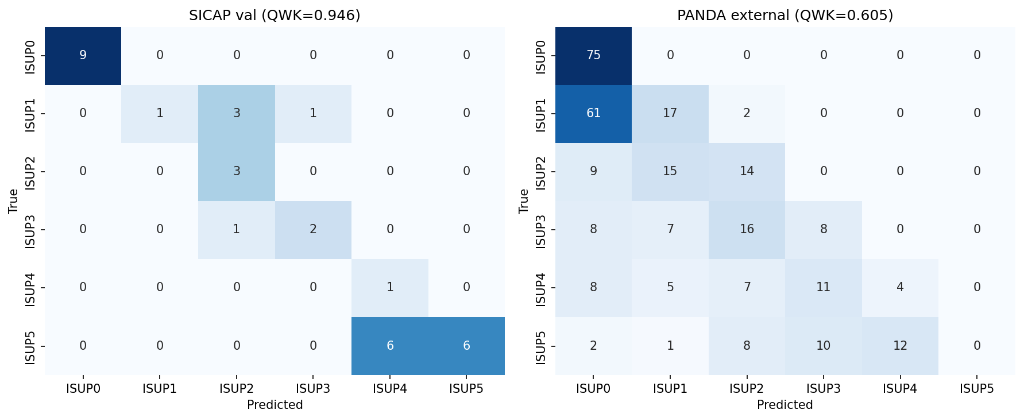
\includegraphics[width=\textwidth]{figure3.png}
\caption{Confusion matrices for the five-fold ensemble using default rounding. Left: 33 held-out SICAPv2 biopsies (QWK = 0.946). Right: 300 PANDA external biopsies (QWK = 0.605).}
\label{fig:confusion_matrices}
\end{figure}

The PANDA confusion matrix highlights both a strength and a serious failure mode. All 75 benign biopsies were predicted as benign, corresponding to 100\% specificity for cancer detection. However, 88 of the 225 malignant biopsies were also classified as benign, giving a cancer-detection sensitivity of 60.9\% (137/225). Most of these false-negative cases were ISUP 1 (61 of 80), but 18 belonged to ISUP 3--5. Errors were strongly directional: among the 182 misgraded biopsies, 180 were assigned a lower grade than the reference, and none of the 33 ISUP 5 biopsies was classified correctly. Despite this zero recall, the ISUP 5 one-versus-rest AUROC was 0.912, the highest among the grade groups. This combination is consistent with useful ranking information accompanied by a downward shift in the regression scores relative to the decision thresholds. It does not establish reliable detection of high-grade disease, and the external results must not be interpreted as evidence of clinical safety.


\subsection{Ablation Study: Pooling and Graph Contributions}
We compared six model variants on the held-out SICAPv2 and PANDA cohorts (Table 6). V1 and V2 implement the patch-percentage rule using the linear probes: the grade is derived from Gleason patterns occupying more than 5\% of malignant patches, using the coarse view alone for V1 and the average of both views for V2. V3 combines graph-transformer layers with mean pooling, whereas V4 uses LRA pooling without graph layers. These two variants were each trained once on the full 366-slide development pool for 30 epochs, without early stopping or a learning-rate schedule. V5a is the best single-fold model from the main cross-validation, and V5b is the corresponding five-fold ensemble. Because V3 and V4 used a different training protocol from V5a and V5b, and because V3 and V4 differ in both graph processing and pooling, this experiment is not a fully factorial ablation.


\begin{table}[H]
\centering
\small
\renewcommand{\arraystretch}{1.15}
\caption{Ablation results on the held-out SICAPv2 cohort ($n = 33$) and PANDA external cohort ($n = 300$). Values are QWK with default rounding and bootstrap 95\% confidence intervals.}
\label{tab:ablation}
\begin{tabularx}{\textwidth}{lXcc}
\toprule
\textbf{Variant} & \textbf{Configuration} & \textbf{SICAPv2 held-out QWK (95\% CI)} & \textbf{PANDA external QWK (95\% CI)} \\
\midrule
V1 & Patch-percentage rule (coarse scale) & 0.642 (0.363--0.828) & 0.346 (0.235--0.456) \\
V2 & Patch-percentage rule, both views averaged & 0.335 (0.012--0.623) & 0.423 (0.310--0.529) \\
V3 & Graph layers + mean pooling & 0.865 (0.696--0.958) & 0.317 (0.264--0.367) \\
V4 & LRA pooling only (no graph layers) & 0.946 (0.891--0.976) & 0.681 (0.608--0.745) \\
V5a & Full model, single best fold & 0.943 (0.878--0.980) & 0.669 (0.596--0.735) \\
V5b & Full model, five-fold ensemble & \textbf{0.946 (0.891--0.977)}$^\dagger$ & \textbf{0.605 (0.531--0.673)} \\
\bottomrule
\end{tabularx}
\end{table}

The results show a substantial association between the pooling operator and external performance. V3, which applies graph-transformer message passing followed by mean pooling, achieved an internal QWK of 0.865 but an external QWK of 0.317, the lowest among the learned variants and below the patch-percentage baseline. V4, which uses LRA pooling without graph layers, reached the highest external QWK (0.681); the full model with LRA pooling achieved 0.669 for its best single fold. These results indicate that LRA pooling, rather than graph message passing, was the component associated with stronger cross-site stability in this set of experiments. The V3--V5a contrast points to the pooling operation as a plausible contributor, although the different training protocols prevent a causal interpretation. One possible explanation is that learned latent queries can emphasize selected tissue regions, whereas mean pooling weights all nodes uniformly. This explanation remains untested. Importantly, graph message passing did not provide an external generalization advantage over LRA pooling alone: V4 matched or exceeded the full graph model on PANDA, and the five-fold full-model ensemble (0.605) fell below the best single fold (0.669).


\subsection{Comparison of Pretrained Encoder Backbones}
We assessed the contribution of the patch encoder by replacing UNI with five ImageNet-pretrained backbones: EfficientNet-B0 \cite{ref28}, ConvNeXt-Tiny \cite{ref29}, ResNet-50 \cite{ref30}, ViT-B/16 \cite{ref23}, and DenseNet-121 \cite{ref31}. Each encoder was frozen, received 224$\times$224 images, and was paired with the same graph and pooling architecture. Each configuration was trained once on the development pool for 30 epochs. Table 7 reports the maximum held-out SICAPv2 QWK observed across those epochs.


\begin{table}[H]
\centering
\small
\renewcommand{\arraystretch}{1.15}
\caption{Comparison of frozen encoders within the GradeFormer graph-and-pooling architecture on the held-out SICAPv2 cohort ($n = 33$).}
\label{tab:encoder_comparison}
\begin{tabularx}{\textwidth}{lXcc}
\toprule
\textbf{Encoder backbone} & \textbf{Pretraining domain} & \textbf{Embedding dim ($D$)} & \textbf{Held-out SICAPv2 QWK} \\
\midrule
\textbf{UNI (ViT-L/16)} & Histopathology ($>$100 M patches) & 1024 & \textbf{0.964} \\
ConvNeXt-Tiny & Natural images (ImageNet) & 768 & 0.925 \\
EfficientNet-B0 & Natural images (ImageNet) & 1280 & 0.921 \\
ViT-B/16 & Natural images (ImageNet) & 768 & 0.896 \\
ResNet-50 & Natural images (ImageNet) & 2048 & 0.892 \\
DenseNet-121 & Natural images (ImageNet) & 1024 & 0.872 \\
\bottomrule
\end{tabularx}
\end{table}

UNI achieved the highest held-out value (0.964), exceeding the strongest ImageNet-pretrained encoder, ConvNeXt-Tiny (0.925), by 0.040. This result is consistent with the potential value of histology-specific pretraining for representing glandular morphology. However, each configuration was run once, and the best epoch was selected using only 33 held-out biopsies. The observed difference is therefore uncertain and was not subjected to a formal statistical test.


\subsection{Statistical Comparison and Computational Cost}
GradeFormer was compared with the patch-percentage baseline (V1) using a paired slide-level bootstrap with 4,000 resamples. For each resample, we calculated the difference in QWK; the one-sided p-value was the proportion of resamples in which the baseline performed at least as well as GradeFormer. As reported in Table 8, no resample favored the baseline in either cohort ($p < 0.001$). The baseline was implemented in this study using the same UNI-based probes and should not be interpreted as a reproduction of a previously published system.


\begin{table}[H]
\centering
\small
\setlength{\tabcolsep}{4pt}
\renewcommand{\arraystretch}{1.15}
\caption{Paired bootstrap comparison of GradeFormer and the patch-percentage baseline using 4,000 resamples and default-rounding predictions.}
\label{tab:bootstrap_significance}
\begin{tabularx}{\textwidth}{p{2.8cm}CCCCC}
\toprule
\textbf{Evaluation cohort} & \textbf{Sample size ($n$)} & \textbf{QWK (GradeFormer)} & \textbf{QWK (baseline)} & \textbf{$\Delta$QWK (point / bootstrap mean)} & \textbf{One-sided bootstrap $p$} \\
\midrule
SICAPv2 held-out & 33 & 0.946 & 0.642 & +0.304 / +0.309 & $< 0.001$ \\
PANDA external & 300 & 0.605 & 0.346 & +0.259 / +0.260 & $< 0.001$ \\
\bottomrule
\end{tabularx}
\end{table}

Table 9 summarizes parameter counts and inference latency for the slide-level components on a single T4 GPU. Latency was estimated from ten forward passes using batches of four held-out SICAPv2 graphs (approximately 131 nodes per graph), following two warm-up passes; elapsed time was divided by the number of graphs. The measurement excludes UNI feature extraction because the foundation-model embeddings were generated once offline and cached, as is common in feature-based MIL pipelines. Feature extraction remains part of the end-to-end workflow and was not timed here. Larger graphs, including PANDA graphs with an average of approximately 399 nodes, are expected to require more computation.


\begin{table}[H]
\centering
\small
\renewcommand{\arraystretch}{1.15}
\caption{Parameter counts and slide-level inference latency on one NVIDIA T4 GPU.}
\label{tab:parameter_latency}
\begin{tabularx}{\textwidth}{lCcX}
\toprule
\textbf{Component} & \textbf{Parameters (M)} & \textbf{Latency (ms / slide)} & \textbf{Role} \\
\midrule
Patch encoder (UNI ViT-L/16, frozen) & 303.35 & Precomputed* & Offline feature extraction (cached) \\
Graph transformer + LRA (proposed) & 11.23 & 1.47 & Slide-level model \\
Graph + mean pooling (V3) & 10.12 & 1.11 & Ablation \\
LRA pooling only (V4) & 1.78 & 0.46 & Ablation \\
\bottomrule
\end{tabularx}
\end{table}


\subsection{Multi-Seed Robustness and Pooling Analysis}
To examine sensitivity to initialization, we repeated five-fold training with seed 123 using LRA pooling, seed 42 using LRA pooling, and seed 777 using mean pooling. These experiments followed a common protocol: a maximum of 30 epochs, cosine scheduling without warm-up, early-stopping patience of five epochs, and retention of the last three improving checkpoints per fold as snapshots. In this set of runs, each slide was treated as an independent group during fold construction; consequently, biopsies from the same SICAPv2 patient could be assigned to different folds. This affects the internal training and stopping procedure but not the independent PANDA evaluation. Table 10 reports PANDA QWK with default rounding for the best-checkpoint and snapshot ensembles.


\begin{table}[H]
\centering
\small
\renewcommand{\arraystretch}{1.15}
\caption{Multi-seed external evaluation on PANDA ($n = 300$) by training seed and pooling operator, using default rounding and bootstrap 95\% confidence intervals.}
\label{tab:multi_seed}
\begin{tabularx}{\textwidth}{llcc}
\toprule
\textbf{Training seed} & \textbf{Pooling} & \textbf{Models in ensemble} & \textbf{PANDA QWK (95\% CI)} \\
\midrule
42 & LRA & 5 (best per fold) & 0.623 (0.552--0.691) \\
42 & LRA & 15 (with snapshots) & 0.636 (0.567--0.701) \\
123 & LRA & 5 (best per fold) & 0.690 (0.623--0.755) \\
123 & LRA & 15 (with snapshots) & 0.609 (0.542--0.674) \\
Mean of LRA seeds 42 and 123 & LRA & N/A & 0.657 $\pm$ 0.034 \\
777 & Mean (negative control) & 5 (best per fold) & 0.208 (0.164--0.253) \\
777 & Mean (negative control) & 15 (with snapshots) & 0.196 (0.155--0.240) \\
All seeds combined & LRA + mean & 45 & 0.503 (0.439--0.565) \\
\bottomrule
\end{tabularx}
\end{table}

The two LRA-pooled runs achieved PANDA QWK values of 0.623 and 0.690, giving a mean of 0.657 (SD 0.034, n = 2). The mean-pooled run achieved 0.208, consistent with the poor external result observed for V3 in Section 4.4. Because the mean-pooling experiment also used a different random seed, the comparison does not isolate the effect of pooling. Nevertheless, the difference between the two LRA runs (0.07 QWK) was substantially smaller than the gap between LRA and mean pooling in these experiments. Snapshot ensembles did not yield a consistent improvement: they modestly increased QWK for seed 42 but reduced it for seed 123 (from 0.690 to 0.609). Combining LRA- and mean-pooled models reduced the ensemble QWK to 0.503, providing no support for mixing these pooling configurations.


\subsection{Error Severity and Uncertainty-Aware Review}
Not all grading errors have the same clinical significance. A one-grade difference between adjacent categories may occur in routine interobserver assessment, whereas failure to recognize high-grade disease could have more serious consequences. Table 11 groups predictions by the absolute difference between predicted and reference grades.


\begin{table}[H]
\centering
\small
\setlength{\tabcolsep}{4pt}
\renewcommand{\arraystretch}{1.15}
\caption{Error severity for the GradeFormer ensemble on the PANDA external cohort and held-out SICAPv2 cohort, using default rounding.}
\label{tab:error_severity}
\begin{tabularx}{\textwidth}{llCCc}
\toprule
\textbf{Error tier} & \textbf{Absolute grade diff.} & \textbf{PANDA ext. ($n = 300$)} & \textbf{SICAPv2 held-out ($n = 33$)} & \textbf{Interpretation} \\
\midrule
Exact agreement & $|$error$| = 0$ & 39.3\% (118/300) & 66.7\% (22/33) & Agreement with reference \\
Adjacent grade & $|$error$| = 1$ & 39.0\% (117/300) & 30.3\% (10/33) & Within typical inter-observer range \\
Moderate discrepancy & $|$error$| = 2$ & 11.0\% (33/300) & 3.0\% (1/33) & Clinically relevant \\
Major discrepancy & $|$error$| \ge 3$ & 10.7\% (32/300) & 0.0\% (0/33) & Severe; target for review \\
\midrule
\textbf{Exact or adjacent} & \textbf{$|$error$| \le 1$} & \textbf{78.3\% (235/300)} & \textbf{97.0\% (32/33)} & \textbf{Combined agreement} \\
\bottomrule
\end{tabularx}
\end{table}

On PANDA, 78.3\% of predictions were either exact (39.3\%) or one grade away (39.0\%), while 10.7\% differed from the reference by at least three grades. Every major and moderate discrepancy was an under-grade. Exact-or-adjacent agreement is sometimes used to contextualize algorithmic disagreement relative to pathologist variability \cite{ref4}, but the strong downward bias observed here means that the 78.3\% figure should not be interpreted as equivalence to pathologist performance. We also calculated, for each biopsy, the standard deviation of the rounded grades predicted by the five fold models. Its association with absolute grading error was weak (Pearson $r = 0.283$, n = 300; Part 2 notebook, Analysis 3). Fold disagreement may help identify some cases for review, but this correlation is too modest to support it as a reliable triage mechanism; no referral threshold or workload was evaluated.


\subsection{Exploratory Interpretability Analyses}
We conducted three exploratory analyses to examine model behavior: slide-level LRA attention maps, patch-level LIME attributions \cite{ref32}, and per-grade discrimination on the external cohort.


\begin{figure}[H]
\centering
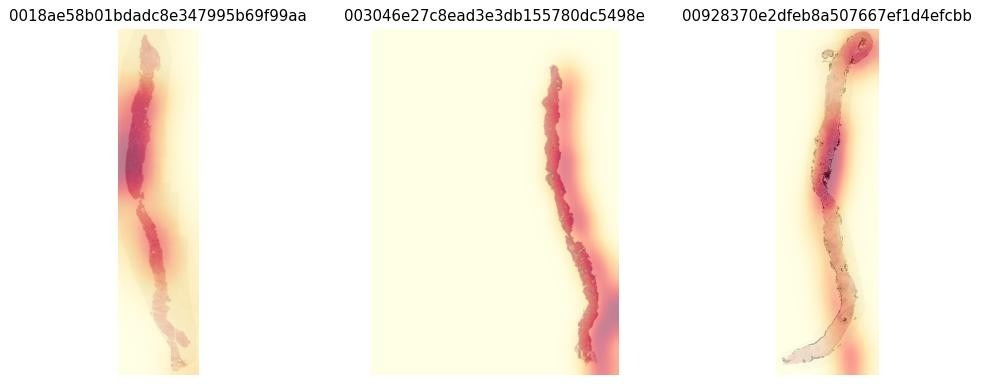
\includegraphics[width=0.85\textwidth]{figure4.png}
\caption{LRA cross-attention maps from the best single-fold model (fold 3), overlaid on three PANDA needle biopsies. The panels show reference grades ISUP 0 (left; benign), ISUP 1 (middle; Gleason 3+3), and ISUP 4 (right; Gleason 4+4). Attention weights were averaged across the 128 latent queries and all heads of the pooling layer, min--max normalized per slide, and rendered as heatmaps over the tissue foreground. Higher attention values are concentrated over malignant glandular areas in the ISUP 1 and ISUP 4 cases.}
\label{fig:attention_heatmaps}
\end{figure}

For Figure 4, attention weights associated with coarse-view nodes were averaged across the 128 latent queries and attention heads, mapped to the patch grid, and smoothed with a Gaussian filter ($\sigma$ = 2 grid cells). Attention was concentrated in selected parts of each core rather than distributed uniformly. The PANDA cases used here did not have region-level annotations available in the analysis pipeline, so correspondence between high-attention regions and carcinoma could not be assessed. An attempted concordance analysis using held-out SICAPv2 patch annotations produced no evaluable slides. The attention maps are therefore qualitative illustrations only.


\begin{figure}[H]
\centering
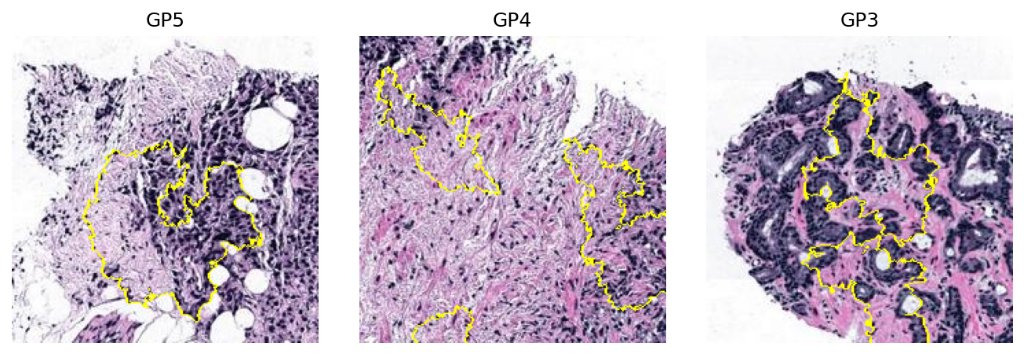
\includegraphics[width=\textwidth]{figure5.png}
\caption{LIME superpixel attributions for the GP3/GP4/GP5 linear probe on one held-out SICAPv2 patch from each class (600 perturbation samples; six superpixels per patch). Positive attributions (green boundaries) indicate image regions that support the predicted Gleason pattern, whereas negative attributions (red boundaries) oppose it. Regions supporting GP3 coincide with discrete, well-formed glands; those for GP4 cover fused glandular networks; and those for GP5 track solid sheets with lost glandular architecture.}
\label{fig:lime}
\end{figure}

Figure 5 presents LIME explanations for one patch from each Gleason pattern. The highlighted regions appear over glandular and epithelial structures: discrete glands in GP3, fused or cribriform architecture in GP4, and solid epithelial regions in GP5. These three examples are insufficient to support a general conclusion about model behavior. In addition, LIME explains the patch-level probe rather than the complete slide-level GradeFormer model, so the results should be interpreted as illustrative.


\begin{figure}[H]
\centering
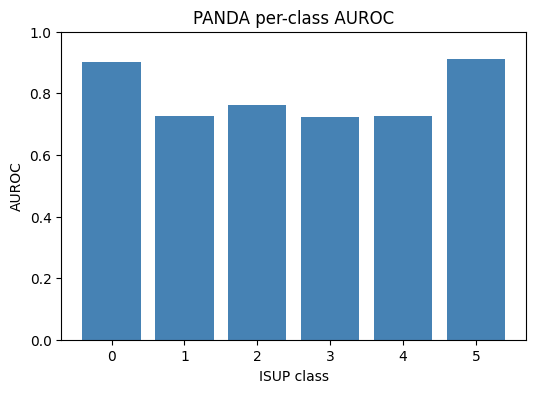
\includegraphics[width=0.7\textwidth]{figure6.png}
\caption{One-versus-rest AUROC for each ISUP grade on the PANDA external cohort, calculated from distance-derived pseudo-probabilities based on the ensemble continuous grade prediction. AUROC was highest for the extreme categories, ISUP 0 (0.902) and ISUP 5 (0.912), and ranged from 0.724 to 0.763 across intermediate grades 1--4.}
\label{fig:panda_auroc}
\end{figure}

Figure 6 shows a U-shaped pattern in one-versus-rest discrimination. AUROC was highest for benign tissue (0.902) and ISUP 5 (0.912), whereas values for ISUP 1--4 ranged from 0.724 to 0.763. Intermediate grades were less readily separated, consistent with the difficulty of distinguishing neighboring Gleason patterns. The high ISUP 5 AUROC does not contradict its zero recall: AUROC measures ranking across thresholds, whereas the reported recall reflects the selected decision threshold. The combination is consistent with a downward displacement of the predicted scores relative to the grade cut-points, but does not demonstrate that a clinically usable threshold is available.


\section{Discussion and Limitations}
This study evaluated whether combining two relative patch scales, slide-level graph structure, latent-query pooling, and ordinal regression could support transfer between prostate histopathology cohorts. GradeFormer was developed using 122 SICAPv2 biopsies and 244 Gleason2019 cores and evaluated without adaptation on 300 PANDA biopsies from two centers. The external QWK was 0.605 with default rounding and 0.586 with the OOF-fitted cut-points, compared with 0.346 for the patch-percentage baseline. These values remain well below the held-out SICAPv2 results (QWK 0.946--0.952). External accuracy was 39.3\%, and the errors were strongly biased toward lower grades. The model is not suitable for clinical use in its current form.

The most consistent pattern across the ablation and multi-seed experiments concerns the pooling operation. Mean-pooled configurations achieved low external QWK values (0.317 in the ablation and 0.208 and 0.196 in the multi-seed experiment), whereas LRA-pooled configurations achieved values between 0.605 and 0.690. These results associate LRA pooling with better cross-site stability than mean pooling. Content-dependent aggregation may allow the slide representation to emphasize selected tissue regions, but the experiments do not establish why the difference occurred. In particular, we did not show that mean pooling propagates scanner- or stain-specific signals. The comparisons were not fully factorial, and the seed and pooling operator changed together in the multi-seed negative control. A controlled study using identical training protocols, multiple seeds, and feature-level domain analyses would be needed to test the proposed explanation.

The graph component did not provide a measurable external generalization advantage over LRA pooling alone. The LRA-only model, with 1.78 M parameters, matched or exceeded the full graph model, which contains 11.23 M trainable parameters, on PANDA and achieved the same held-out internal QWK. Spatial and cross-scale message passing may require more diverse training data to be beneficial, or differences in patch resolution across cohorts may limit the value of the current graph construction. The available results do not support the claim that the graph layers improve cross-institutional grading. LRA pooling alone should therefore be treated as a strong, more compact baseline for subsequent comparisons.

The external error profile raises a more important concern than the overall QWK alone. Although all 75 benign PANDA biopsies were classified as benign, benign precision was only 0.460 because 88 malignant biopsies were also assigned grade 0. Cancer-detection sensitivity was 60.9\% (137/225), and no ISUP 5 biopsy was correctly identified (recall 0/33). The high AUROC for ISUP 5, together with the predominance of under-grading, is compatible with a domain-dependent shift in the regression scores relative to the decision thresholds. Cut-points estimated from the development cohort did not correct this shift. Calibration using a small labeled sample from the target institution or a suitable unsupervised score-alignment strategy could be investigated, but neither approach was evaluated in this study. Fold-ensemble disagreement was only weakly associated with error ($r = 0.283$) and should not be considered a substitute for pathologist review.

Several limitations constrain the interpretation of these findings:

\begin{itemize}[leftmargin=1.8em, itemsep=3pt, parsep=0pt]
  \item \textbf{Limited internal test size.} The held-out SICAPv2 cohort contains 33 biopsies from 19 patients, including 12 ISUP 5 cases. Confidence intervals are consequently broad, and a small number of observations can materially affect the internal estimates.
  \item \textbf{Auxiliary pseudo-labels and a non-standard grade mapping.} The 244 Gleason2019 cores were assigned grades using a percentage rule applied to tile-level majority classes, which introduces unquantified label noise. The pattern-to-grade lookup also differs from the ISUP definition for several combinations (Section 3.3). Cross-validation performance therefore combines SICAPv2 reference grades with Gleason2019 pseudo-grades.
  \item \textbf{External cohort size and sampling.} The PANDA evaluation used the first 300 entries in the public training metadata rather than a random, stratified, or consecutive sample. Its reference labels were those provided in the public training set. No more than 384 tissue tiles were retained per slide. Further assessment on larger, consecutive biopsy cohorts from additional institutions is required.
  \item \textbf{Differences in physical scale.} The two views are defined relative to each cohort's source patch, and the field of view of a 512$\times$512 region differs across SICAPv2, Gleason2019, and PANDA. This variation may contribute to domain shift; consequently, the 10$\times$ and 20$\times$ labels represent relative zoom levels rather than calibrated optical magnifications.
  \item \textbf{Selection of the reported discretization.} The analysis workflow selected the better-performing option between default rounding and OOF-fitted cut-points after examining PANDA results. Both values are reported, but the external QWK of 0.605 is more optimistic; 0.586 is the result obtained with the OOF-fitted thresholds specified independently of PANDA.
  \item \textbf{Ablation and multi-seed design.} The ablation variants did not share identical training protocols. In the multi-seed experiment, seed and pooling method changed together, and only two LRA seeds and one mean-pooling seed were evaluated. The encoder comparison also selected the best epoch using the held-out cohort, leading to optimistic estimates.
  \item \textbf{Frozen foundation encoder.} UNI was used as a frozen feature extractor because of the available single-GPU resources. Parameter-efficient adaptation methods, including low-rank adaptation and prompt tuning, were not investigated and may warrant future study.
  \item \textbf{Qualitative interpretability.} Attention maps and LIME attributions were assessed visually on a small number of examples. The planned quantitative comparison with patch-level annotations yielded no evaluable slides, and dense pathologist delineations were not available. The interpretability results should therefore be viewed as exploratory.
\end{itemize}


\section{Conclusion}
GradeFormer combines frozen UNI features from two relative patch scales, a spatial and cross-scale slide graph, LRA pooling, and continuous ordinal regression for ISUP grading of prostate biopsies. On 300 PANDA biopsies evaluated without fine-tuning, the five-fold ensemble achieved QWK 0.605 with default rounding and 0.586 with OOF-fitted cut-points, compared with 0.346 for the patch-percentage baseline ($\Delta$QWK = +0.259; $p < 0.001$). The principal empirical finding is that LRA pooling was associated with better external stability than mean pooling, while graph message passing did not improve generalization over LRA pooling alone. The external cohort also exposed a clinically important downward bias: 88 of 225 malignant biopsies were classified as benign, and none of the 33 ISUP 5 cases was correctly graded. Target-site calibration, standard-conforming auxiliary labels, and validation on larger consecutive cohorts are necessary before clinical utility can be considered.


\section*{Declarations}
\textbf{Ethics approval and consent to participate:} The study used publicly available, de-identified image datasets (SICAPv2, Gleason2019, and PANDA). No new patient data were collected, no participants were contacted, and no identifiable personal information was accessed. Additional ethical approval was therefore not sought.

\textbf{Funding:} This research was supported by the Basic Science Research Program through the National Research Foundation of Korea (NRF), funded by the Ministry of Education.

\textbf{Competing interests:} The authors declare that they have no competing financial interests or personal relationships that could have influenced the work reported in this paper.

\textbf{Data availability:} All datasets analyzed in this study are publicly available. SICAPv2 is described in \cite{ref12} and distributed through Mendeley Data; Gleason2019 is available through the Grand Challenge platform \cite{ref5}; and PANDA is available through Kaggle \cite{ref6}.

\textbf{Code availability:} Source code, precomputed graph structures, and trained model weights are publicly available at \url{https://github.com/AMINURJOY/GradeFormer}.

\textbf{Use of generative AI:} During manuscript preparation, the authors used Claude (Anthropic) and ChatGPT (OpenAI) for language editing and editorial refinement. The authors reviewed and revised the resulting text and accept responsibility for all statements and for the final manuscript.


% --- Bibliography ---
\bibliographystyle{IEEEtran}
\bibliography{references}

\end{document}
